\chapter{Anexo}
\label{ch:anexo}

\section{Instalando CentOS 7}
\label{sec:instalando_centos}

La instalación de CentOS se basa en el instalador Anaconda, que ya viene siendo usado en Red Hat Enterprise Linux y Fedora. Difiere de otros instaladores, en que en lugar de ser lineal, presenta al usuario una \emph{landing screen}, en la cual se encuentran las diferentes preguntas que típicamente se realizan durante una instalación: El particionado de los discos, idioma, distribución de teclado, paquetes a instalar\ldots La siguiente captura muestra dicha pantalla:

\begin{figure}[ht!]
  \centering
  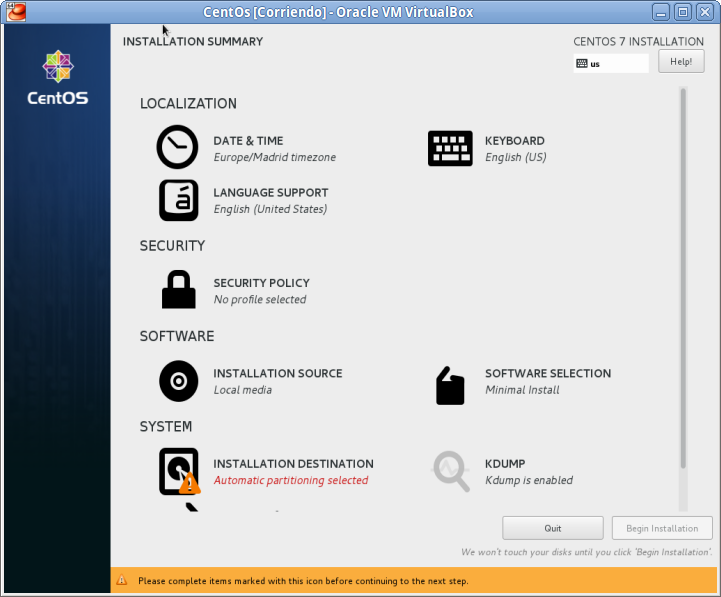
\includegraphics[scale=0.55]{img/anaconda1.png}
  \caption{\label{fig:label} Pantalla principal del instalador Anaconda en CentOS}
\end{figure}

Algunos de los apartados son bastante sencillos y se explican ellos mimsos, así que no incluiré capturas de los mismos. 

\subsection{Localización}
\label{subsec:localizacion}

\subsubsection{Fecha y hora}
\label{subsec:fechahora}

Éste apartado es muy similar al de otros instaladores. Un mapa del planeta aparecerá, dónde podremos seleccionar nuestra ciudad. Acorde a la selección, se ajustará la hora del sistema. Es posible también desactivar NTS, y introducir tanto la fecha como la hora de forma manual.

\subsubsection{Teclado}
\label{subsec:teclado}

Bastante simple también. Aparecerán dos cuadros, uno a la izquierda y otro a la derecha. En la parte inferior del panel izquierdo habrá una lista de botones, que corresponden a Añadir, Quitar, Mover arriba y Mover abajo. Cuando seleccionemos Añadir, aparecerá una lista de idiomas, y las distribuciones de cada idioma una vez se haya seleccionado uno.

En el derecho, simplemente, se podrá probar la distribución de teclado seleccionada.

\subsubsection{Soporte de idiomas}
\label{subsec:soportedeidiomas}

La pantalla de soporte de idiomas es casi exactamente la misma que la primera que encontramos nada más arrancar el instalador, con la única diferencia que en lugar de escoger un único idioma, podemos ir marcando varios, para que luego se instale soporte para todos aquellos idiomas marcados.

\subsection{Discos}
\label{subsec:discos}

Éste es el único apartado \emph{obligatorio} para completar la instalación; todos los demás apartados pueden dejarse con los valores por defecto. Una vez accedemos al apartado, se nos presenta la siguiente pantalla:

\begin{figure}[ht!]
  \centering
  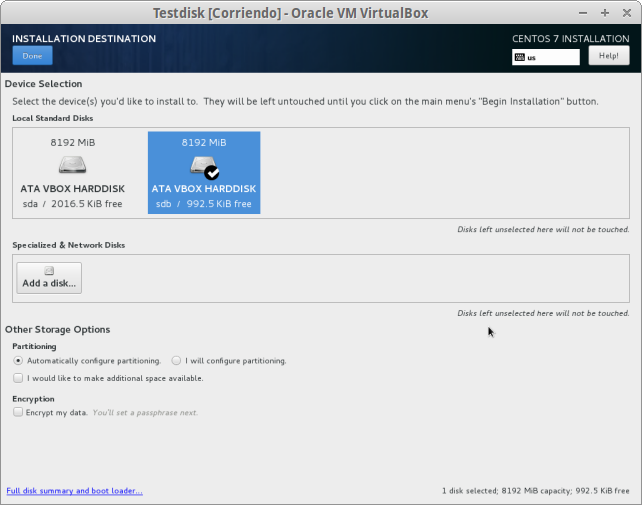
\includegraphics[scale=0.55]{centos-disk1.png}
  \caption{\label{fig:diskselect} Selección de discos}
\end{figure}

\begin{figure}[ht!]
  \centering
  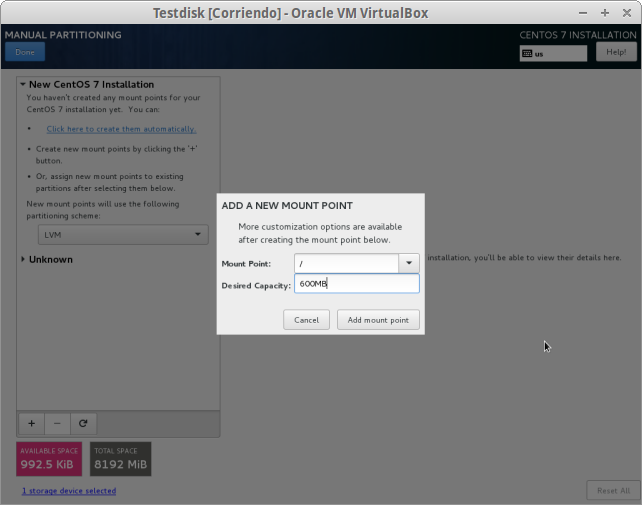
\includegraphics[scale=0.55]{centos-disk2.png}
  \caption{\label{fig:add_mpoint} Añadiendo punto de montaje}
\end{figure}

\begin{figure}[ht!]
  \centering
  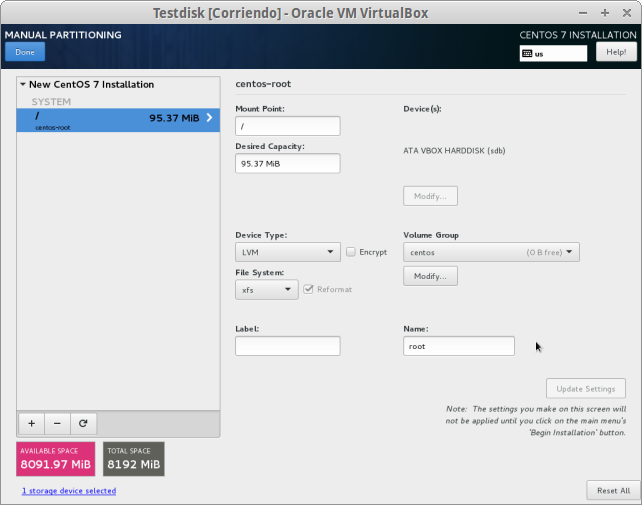
\includegraphics[scale=0.55]{centos-disk3.png}
  \caption{\label{fig:edit_mpoint} Editando punto de montaje}
\end{figure}

\clearpage

\subsection{Continuando la instalación}
\label{subsec:continuando}

Una vez realizado el particionamiento de los discos, la instalación se iniciará, y deberemos editar la contraseña del usuario root, y crear un usuario adicional. 


\section{Trabajando remotamente}
\label{sec:remote}

Dadas las circunstancias del proyecto (No dispongo del hardware físico en el Puig), y que ahora sólo voy aproximadamente ocho horas a la semana a la Bastida, he tenido que buscarme la vida para poder trabajar con las máquinas virtuales en el Puig.

La solución que detallaré ahora a continuación no es muy complicada, pero todo gira en torno a que La Bastida tenga conexión a Internet. Si no puedo llegar hasta su proxy, no puedo trabajar. Una vez dicho esto, lo primero que tengo que hacer para poder acceder a la máquina de la red local de la Bastida donde está instalada la interfaz web del motor, es convertir a mi portátil en un proxy SOCKS.\@Ésto lo puedo hacer mediante el siguiente túnel SSH:

\begin{TMterminal}{}{}{Creando el túnel}
  ssh -D 10080 enrique@ieslabastida.xtec.cat -p 2209
\end{TMterminal}

Mientras la sesión SSH siga activa, mi portátil estará actuando como un proxy SOCKS.\@Si configuro Firefox con dicho proxy como en la siguiente captura: 

\begin{figure}[ht!]
  \centering
  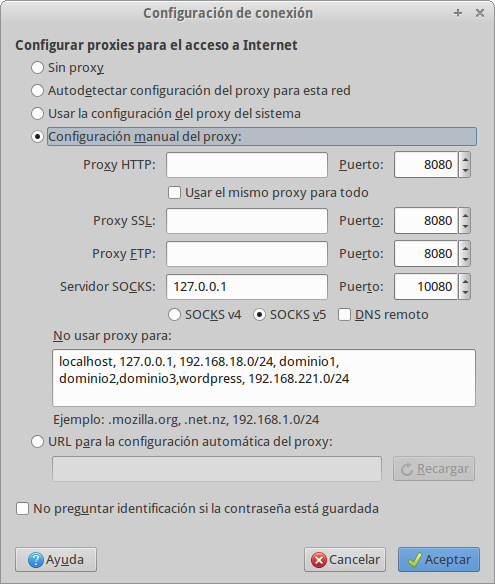
\includegraphics[scale=0.55]{proxyconf.png}
  \caption{\label{fig:Proxy} Configuración del proxy en Firefox}
\end{figure}

Todo el tráfico pasará por el puerto 10080 de mi portátil, que no es ni más ni menos un túnel SSH al Proxy de la Bastida, que atenderá la petición, y me permitirá conectarme al portal de administración.

\subsection{Consola remota mediante el proxy SOCKS}
\label{subsec:consola}

oVirt permite utilizar un cliente de consola remota para conectarse a las máquinas virtuales, y trabajar con el escritorio remoto. Ésto se hace mediante ficheros con extensión $.$vv que permiten a un programa como remote-viewer conectarse. El único problema, es que éste programa no incluye configuración de red, ni la distribución que utilizo (Xubuntu 15.10) incluye configuración global del proxy. La solución a éste problema radica entonces en la librería \textbf{tsocks}, que intercepta todo el tráfico saliente, y lo re-envía a un servidor SOCKS.\@Está pensado para aplicaciones que por defecto no tratan bien con servidores proxy SOCKS.

La siguiente figura muestra la breve configuración (sólo dos líneas) necesarias para hacer que tsocks mande el tráfico por el mismo proxy SOCKS que utilizamos antes:

\begin{TMterminal}{}{}{Configurando tsocks}
  server      = 127.0.0.1
  server_port = 10080
\end{TMterminal}

Una vez editado el fichero de configuración /etc/tsocks, ya podemos ejecutar cualquier programa tal que \texttt{tsocks} \emph{programa}, y todo el tráfico de red que éste genere irá a pasar al servidor SOCKS.







